\PassOptionsToPackage{unicode=true}{hyperref} % options for packages loaded elsewhere
\PassOptionsToPackage{hyphens}{url}
%
\documentclass[]{article}
\usepackage{lmodern}
\usepackage{amssymb,amsmath}
\usepackage{ifxetex,ifluatex}
\usepackage{fixltx2e} % provides \textsubscript
\ifnum 0\ifxetex 1\fi\ifluatex 1\fi=0 % if pdftex
  \usepackage[T1]{fontenc}
  \usepackage[utf8]{inputenc}
  \usepackage{textcomp} % provides euro and other symbols
\else % if luatex or xelatex
  \usepackage{unicode-math}
  \defaultfontfeatures{Ligatures=TeX,Scale=MatchLowercase}
\fi
% use upquote if available, for straight quotes in verbatim environments
\IfFileExists{upquote.sty}{\usepackage{upquote}}{}
% use microtype if available
\IfFileExists{microtype.sty}{%
\usepackage[]{microtype}
\UseMicrotypeSet[protrusion]{basicmath} % disable protrusion for tt fonts
}{}
\IfFileExists{parskip.sty}{%
\usepackage{parskip}
}{% else
\setlength{\parindent}{0pt}
\setlength{\parskip}{6pt plus 2pt minus 1pt}
}
\usepackage{hyperref}
\hypersetup{
            pdftitle={R Markdown testbed},
            pdfauthor={Rick Gilmore},
            pdfborder={0 0 0},
            breaklinks=true}
\urlstyle{same}  % don't use monospace font for urls
\usepackage[margin=1in]{geometry}
\usepackage{color}
\usepackage{fancyvrb}
\newcommand{\VerbBar}{|}
\newcommand{\VERB}{\Verb[commandchars=\\\{\}]}
\DefineVerbatimEnvironment{Highlighting}{Verbatim}{commandchars=\\\{\}}
% Add ',fontsize=\small' for more characters per line
\usepackage{framed}
\definecolor{shadecolor}{RGB}{248,248,248}
\newenvironment{Shaded}{\begin{snugshade}}{\end{snugshade}}
\newcommand{\AlertTok}[1]{\textcolor[rgb]{0.94,0.16,0.16}{#1}}
\newcommand{\AnnotationTok}[1]{\textcolor[rgb]{0.56,0.35,0.01}{\textbf{\textit{#1}}}}
\newcommand{\AttributeTok}[1]{\textcolor[rgb]{0.77,0.63,0.00}{#1}}
\newcommand{\BaseNTok}[1]{\textcolor[rgb]{0.00,0.00,0.81}{#1}}
\newcommand{\BuiltInTok}[1]{#1}
\newcommand{\CharTok}[1]{\textcolor[rgb]{0.31,0.60,0.02}{#1}}
\newcommand{\CommentTok}[1]{\textcolor[rgb]{0.56,0.35,0.01}{\textit{#1}}}
\newcommand{\CommentVarTok}[1]{\textcolor[rgb]{0.56,0.35,0.01}{\textbf{\textit{#1}}}}
\newcommand{\ConstantTok}[1]{\textcolor[rgb]{0.00,0.00,0.00}{#1}}
\newcommand{\ControlFlowTok}[1]{\textcolor[rgb]{0.13,0.29,0.53}{\textbf{#1}}}
\newcommand{\DataTypeTok}[1]{\textcolor[rgb]{0.13,0.29,0.53}{#1}}
\newcommand{\DecValTok}[1]{\textcolor[rgb]{0.00,0.00,0.81}{#1}}
\newcommand{\DocumentationTok}[1]{\textcolor[rgb]{0.56,0.35,0.01}{\textbf{\textit{#1}}}}
\newcommand{\ErrorTok}[1]{\textcolor[rgb]{0.64,0.00,0.00}{\textbf{#1}}}
\newcommand{\ExtensionTok}[1]{#1}
\newcommand{\FloatTok}[1]{\textcolor[rgb]{0.00,0.00,0.81}{#1}}
\newcommand{\FunctionTok}[1]{\textcolor[rgb]{0.00,0.00,0.00}{#1}}
\newcommand{\ImportTok}[1]{#1}
\newcommand{\InformationTok}[1]{\textcolor[rgb]{0.56,0.35,0.01}{\textbf{\textit{#1}}}}
\newcommand{\KeywordTok}[1]{\textcolor[rgb]{0.13,0.29,0.53}{\textbf{#1}}}
\newcommand{\NormalTok}[1]{#1}
\newcommand{\OperatorTok}[1]{\textcolor[rgb]{0.81,0.36,0.00}{\textbf{#1}}}
\newcommand{\OtherTok}[1]{\textcolor[rgb]{0.56,0.35,0.01}{#1}}
\newcommand{\PreprocessorTok}[1]{\textcolor[rgb]{0.56,0.35,0.01}{\textit{#1}}}
\newcommand{\RegionMarkerTok}[1]{#1}
\newcommand{\SpecialCharTok}[1]{\textcolor[rgb]{0.00,0.00,0.00}{#1}}
\newcommand{\SpecialStringTok}[1]{\textcolor[rgb]{0.31,0.60,0.02}{#1}}
\newcommand{\StringTok}[1]{\textcolor[rgb]{0.31,0.60,0.02}{#1}}
\newcommand{\VariableTok}[1]{\textcolor[rgb]{0.00,0.00,0.00}{#1}}
\newcommand{\VerbatimStringTok}[1]{\textcolor[rgb]{0.31,0.60,0.02}{#1}}
\newcommand{\WarningTok}[1]{\textcolor[rgb]{0.56,0.35,0.01}{\textbf{\textit{#1}}}}
\usepackage{graphicx,grffile}
\makeatletter
\def\maxwidth{\ifdim\Gin@nat@width>\linewidth\linewidth\else\Gin@nat@width\fi}
\def\maxheight{\ifdim\Gin@nat@height>\textheight\textheight\else\Gin@nat@height\fi}
\makeatother
% Scale images if necessary, so that they will not overflow the page
% margins by default, and it is still possible to overwrite the defaults
% using explicit options in \includegraphics[width, height, ...]{}
\setkeys{Gin}{width=\maxwidth,height=\maxheight,keepaspectratio}
\usepackage[normalem]{ulem}
% avoid problems with \sout in headers with hyperref:
\pdfstringdefDisableCommands{\renewcommand{\sout}{}}
\setlength{\emergencystretch}{3em}  % prevent overfull lines
\providecommand{\tightlist}{%
  \setlength{\itemsep}{0pt}\setlength{\parskip}{0pt}}
\setcounter{secnumdepth}{0}
% Redefines (sub)paragraphs to behave more like sections
\ifx\paragraph\undefined\else
\let\oldparagraph\paragraph
\renewcommand{\paragraph}[1]{\oldparagraph{#1}\mbox{}}
\fi
\ifx\subparagraph\undefined\else
\let\oldsubparagraph\subparagraph
\renewcommand{\subparagraph}[1]{\oldsubparagraph{#1}\mbox{}}
\fi

% set default figure placement to htbp
\makeatletter
\def\fps@figure{htbp}
\makeatother

\usepackage{etoolbox}
\makeatletter
\providecommand{\subtitle}[1]{% add subtitle to \maketitle
  \apptocmd{\@title}{\par {\large #1 \par}}{}{}
}
\makeatother

\title{R Markdown testbed}
\providecommand{\subtitle}[1]{}
\subtitle{PSY 525}
\author{Rick Gilmore}
\date{2020-02-04 12:21:48}

\begin{document}
\maketitle

\hypertarget{this-is-a-heading-1}{%
\section{This is a Heading 1}\label{this-is-a-heading-1}}

\hypertarget{this-is-a-heading-2}{%
\subsection{This is a Heading 2}\label{this-is-a-heading-2}}

\hypertarget{this-is-a-heading-3}{%
\subsubsection{This is a Heading 3}\label{this-is-a-heading-3}}

\hypertarget{lists}{%
\section{Lists}\label{lists}}

\hypertarget{not-enumerated}{%
\subsection{Not enumerated}\label{not-enumerated}}

\begin{itemize}
\tightlist
\item
  An item

  \begin{itemize}
  \tightlist
  \item
    A nested item with \textbf{boldface}

    \begin{itemize}
    \tightlist
    \item
      A doubly-nested item with \emph{italics}
    \end{itemize}
  \end{itemize}
\item
  Another item with some \sout{text stricken out}
\item
  URL: \href{https://www.psu.edu}{Penn State Home}
\end{itemize}

\hypertarget{enumerated}{%
\subsection{Enumerated}\label{enumerated}}

\begin{enumerate}
\def\labelenumi{\arabic{enumi}.}
\tightlist
\item
  An enumerated item

  \begin{itemize}
  \tightlist
  \item
    A nested item
  \end{itemize}
\item
  A second enumerated item

  \begin{enumerate}
  \def\labelenumii{\alph{enumii}.}
  \tightlist
  \item
    A nested item with a footnote \footnote{Here is the footnote text.
      Note that it ends up at the end of the document.} marker. Look for
    the text at the end of the document.
  \item
    A second nested item. See how alphabetical enumerated lists work
    like you'd expect.
  \end{enumerate}
\end{enumerate}

\hypertarget{block-quotation}{%
\subsection{Block quotation}\label{block-quotation}}

\begin{quote}
Four score and seven years ago, some famous President spoke infamous
words that would live on throughout history. These words are famous
enough that I want to highlight them with a block quote.
\end{quote}

\hypertarget{make-some-data}{%
\section{Make some data}\label{make-some-data}}

\begin{Shaded}
\begin{Highlighting}[]
\NormalTok{x =}\StringTok{ }\KeywordTok{rnorm}\NormalTok{(}\DataTypeTok{n =} \DecValTok{100}\NormalTok{, }\DataTypeTok{mean =} \DecValTok{0}\NormalTok{, }\DataTypeTok{sd =} \DecValTok{1}\NormalTok{)   }\CommentTok{# N(0,1)}
\NormalTok{y =}\StringTok{ }\KeywordTok{rnorm}\NormalTok{(}\DataTypeTok{n =} \DecValTok{100}\NormalTok{, }\DataTypeTok{mean =} \DecValTok{2}\NormalTok{, }\DataTypeTok{sd =} \FloatTok{0.5}\NormalTok{) }\CommentTok{# N(2, 0.5)}
\end{Highlighting}
\end{Shaded}

\hypertarget{summarize}{%
\subsection{Summarize}\label{summarize}}

\begin{Shaded}
\begin{Highlighting}[]
\KeywordTok{summary}\NormalTok{(x)}
\end{Highlighting}
\end{Shaded}

\begin{verbatim}
##    Min. 1st Qu.  Median    Mean 3rd Qu.    Max. 
## -1.7199 -0.6222  0.2658  0.1589  0.7511  2.0952
\end{verbatim}

\begin{Shaded}
\begin{Highlighting}[]
\KeywordTok{summary}\NormalTok{(y)}
\end{Highlighting}
\end{Shaded}

\begin{verbatim}
##    Min. 1st Qu.  Median    Mean 3rd Qu.    Max. 
##  0.8085  1.7071  2.0136  2.0436  2.4124  3.3837
\end{verbatim}

\hypertarget{histogram}{%
\subsection{Histogram}\label{histogram}}

\begin{Shaded}
\begin{Highlighting}[]
\KeywordTok{hist}\NormalTok{(x)}
\end{Highlighting}
\end{Shaded}

\begin{center}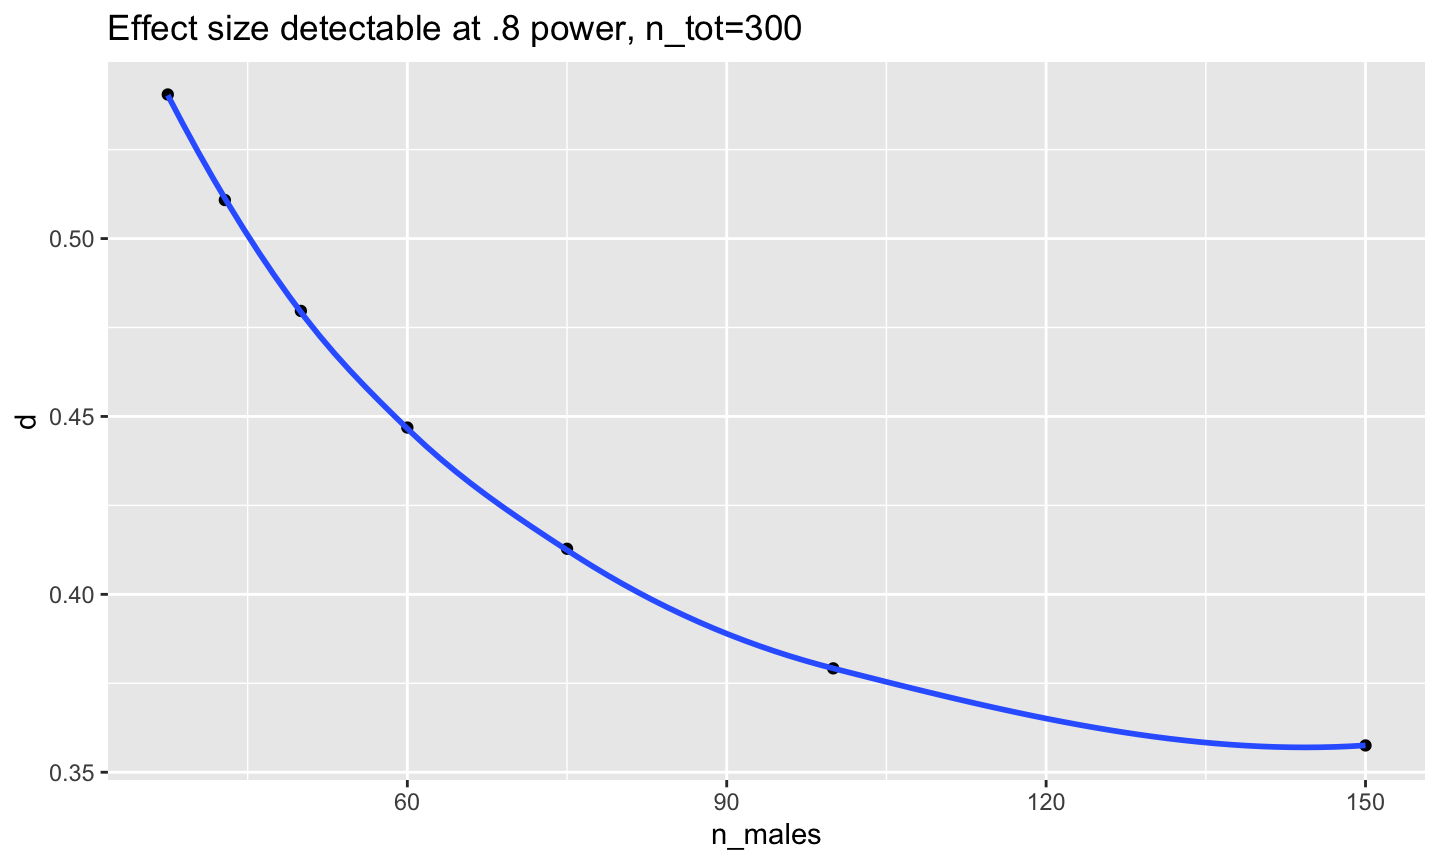
\includegraphics[width=400px]{testbed_files/figure-latex/unnamed-chunk-3-1} \end{center}

\hypertarget{plot}{%
\subsection{Plot}\label{plot}}

\begin{Shaded}
\begin{Highlighting}[]
\KeywordTok{plot}\NormalTok{(x,y)}
\end{Highlighting}
\end{Shaded}

\begin{center}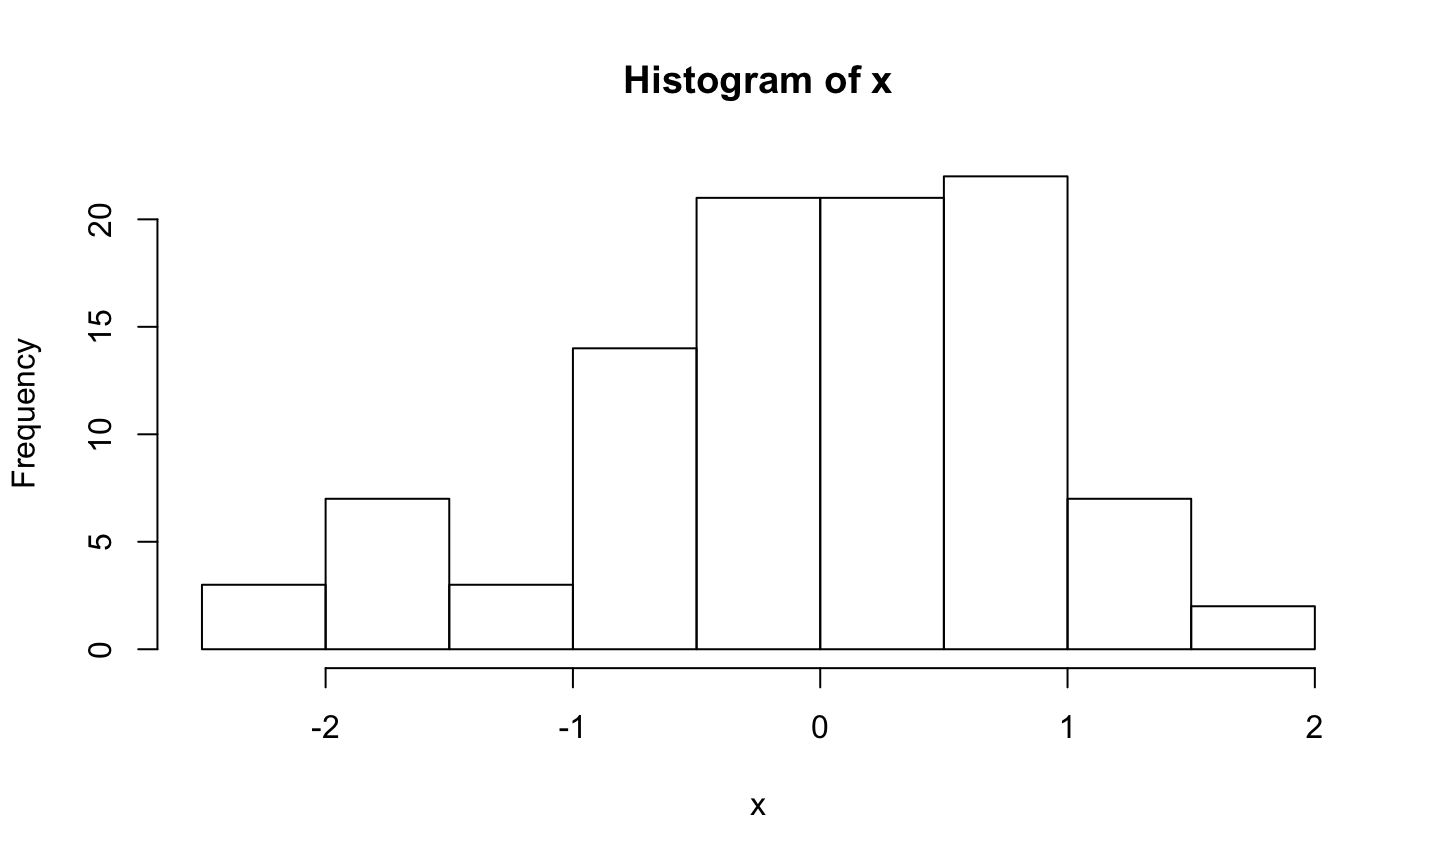
\includegraphics[width=400px]{testbed_files/figure-latex/unnamed-chunk-4-1} \end{center}

\hypertarget{embed-figures-or-videos}{%
\section{Embed figures or videos}\label{embed-figures-or-videos}}

Some of these methods work better than others with a particular output
format.

\hypertarget{from-the-web-using-knitrinclude_graphics.}{%
\subsection{\texorpdfstring{From the web using
\texttt{knitr::include\_graphics()}.}{From the web using knitr::include\_graphics().}}\label{from-the-web-using-knitrinclude_graphics.}}

The \texttt{html\_document} format is fine with using the URL as the
input to \texttt{knitr::include\_graphics()}, but the
\texttt{pdf\_document} format seems to want a local file path, hence the
use of \texttt{download.file()}.

\begin{Shaded}
\begin{Highlighting}[]
\KeywordTok{download.file}\NormalTok{(}\StringTok{"https://nyu.databrary.org/party/6/avatar"}\NormalTok{,}\StringTok{'img/rog.png'}\NormalTok{, }\DataTypeTok{mode =} \StringTok{'wb'}\NormalTok{)}
\NormalTok{knitr}\OperatorTok{::}\KeywordTok{include_graphics}\NormalTok{(}\StringTok{"img/rog.png"}\NormalTok{)}
\end{Highlighting}
\end{Shaded}

\begin{figure}

{\centering 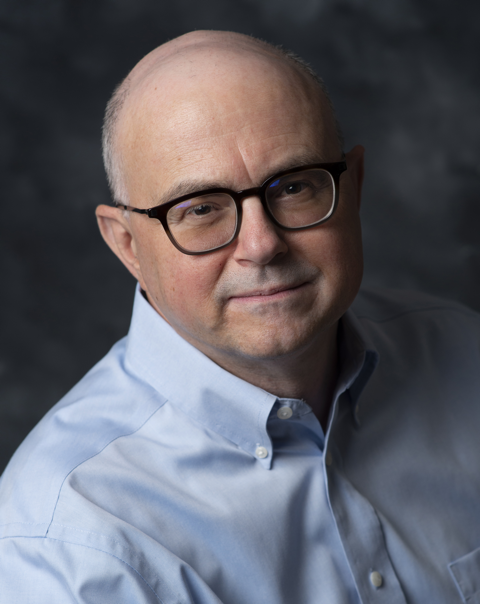
\includegraphics[width=400px]{img/rog} 

}

\caption{Rick's pic from Databrary}\label{fig:rog}
\end{figure}

\hypertarget{from-a-local-file-using-html}{%
\subsection{From a local file using
HTML}\label{from-a-local-file-using-html}}

\hypertarget{from-a-local-file-using-knitrinclude_graphics}{%
\subsection{\texorpdfstring{From a local file using
\texttt{knitr::include\_graphics()}}{From a local file using knitr::include\_graphics()}}\label{from-a-local-file-using-knitrinclude_graphics}}

\begin{Shaded}
\begin{Highlighting}[]
\NormalTok{knitr}\OperatorTok{::}\KeywordTok{include_graphics}\NormalTok{(}\StringTok{"img/sleic.jpg"}\NormalTok{)}
\end{Highlighting}
\end{Shaded}

\begin{center}
\includegraphics[width=400px]{img/sleic} \end{center}

\hypertarget{from-a-local-file-using-markdown-syntax}{%
\subsection{From a local file using Markdown
syntax}\label{from-a-local-file-using-markdown-syntax}}

\begin{figure}
\centering

\includegraphics{img/sleic.jpg}
\caption{SLEIC}
\end{figure}

\hypertarget{from-youtube}{%
\subsection{From YouTube}\label{from-youtube}}

\hypertarget{printing-values-from-r}{%
\section{Printing values from R}\label{printing-values-from-r}}

\begin{Shaded}
\begin{Highlighting}[]
\NormalTok{summ.x =}\StringTok{ }\KeywordTok{summary}\NormalTok{(x)}
\NormalTok{summ.y =}\StringTok{ }\KeywordTok{summary}\NormalTok{(y)}
\KeywordTok{names}\NormalTok{(summ.x) }\CommentTok{# Figure out variable names for indexing}
\end{Highlighting}
\end{Shaded}

\begin{verbatim}
## [1] "Min."    "1st Qu." "Median"  "Mean"   
## [5] "3rd Qu." "Max."
\end{verbatim}

\emph{Index by variable name:} X lies within the range of {[}-1.7198644,
2.0952016{]}.

\emph{Index by numeric index:} The (y-x) difference in means is
1.8846229.

\emph{Calculate and report:} The correlation between x and y is
0.0967532.

\hypertarget{math-equations}{%
\section{Math equations}\label{math-equations}}

\[e=mc^{2}\]

\hypertarget{parameterized-reports}{%
\section{Parameterized reports}\label{parameterized-reports}}

\hypertarget{my-name-is-steve}{%
\subsection{My name is Steve}\label{my-name-is-steve}}

\hypertarget{my-quest-is-to-find-the-grail}{%
\subsection{My quest is to find the
grail}\label{my-quest-is-to-find-the-grail}}

\hypertarget{my-favorite-color-is-blue}{%
\subsection{My favorite color is blue}\label{my-favorite-color-is-blue}}

\hypertarget{footnotes}{%
\section{Footnotes}\label{footnotes}}

\end{document}
